% !TEX program = XeLaTeX
\documentclass{VUMIFPSkursinis}
\usepackage{algorithmicx}
\usepackage{algorithm}
\usepackage{algpseudocode}
\usepackage{amsfonts}
\usepackage{amsmath}
\usepackage{bm}
\usepackage{caption}
\usepackage{color}
\usepackage{float}
\usepackage{graphicx}
\usepackage{listings}
\usepackage{subfig}
\usepackage{wrapfig}

% Titulinio aprašas
\university{Vilniaus universitetas}
\faculty{Matematikos ir informatikos fakultetas}
\department{Programų sistemų katedra}
\papertype{Laboratorinis darbas}
\title{Skrydžių bilietų paieškos sistema}
\titleineng{Plane tickets search system}
\status{2 kurso 4 grupės studentai}
\author{Vardenis Pavardenis}
\secondauthor{Vardenis Pavardenis}
\thirdauthor{Vardenis Pavardenis}
\fourthauthor{Vardenis Pavardenis}
\date{Vilnius – \the\year}

% Nustatymai
% \setmainfont{Palemonas}   % Pakeisti teksto šriftą į Palemonas (turi būti įdiegtas sistemoje)
\bibliography{bibliografija}

\begin{document}
\maketitle

\tableofcontents

\sectionnonum{Įvadas}
...

\section{Vartotojo interfeiso reikalavimai}

\subsection{Dalykinės srities metaforų reikalavimai}

\begin{table}[H]\footnotesize
  \centering
  \caption{Dalykinės srities metaforų reikalavimai}
  {\begin{tabular}{|l|l|} \hline
    Objektas & Metafora \\
    \hline
    \hline
    Vartotojas  & Asmuo, norintis nusipirkti skrydžio bilietą \\
    \hline
    Skrydžių bendrovė  & Įmonė, kuri suteikia skrydžio paslaugą \\
    \hline
    Paieška & Skrydžių bilietų radimas pagal įvestus paieškos kriterijus \\
    \hline
    Rūšiavimas & Maršruto pasirinkimas pagal norimą kriterijų: greitis, kaina, greičio ir kainos santykis \\
    \hline
    Filtravimas & Rezultatų pateikimas pagal norimus kriterijus: persėdimų skaičius, skrydžių bendrovės \\
    \hline
    Kainų žirklės & Kainos amplitudė \\
    \hline
    Užsakymų istorija & Įsigytų skrydžių bilietų peržiūra \\
    \hline
    Skrydžių informacija & Įsigytos kelionės duomenys: data, laikas, oro uostai \\
    \hline
    Paieškos rezultatai & Gautos užklausos rezultatai \\
    \hline
  \end{tabular}}
  \label{tab:table example}
\end{table}

\subsubsection{Formuluojamos užduotys}
Sistemos naudotojo interfeiso formuluojamos užduotys:
\begin{itemize}
  \item Datos įvedimas
  \item Kainos įvedimas
  \item Miestų įvedimas
  \item Esamos informacijos peržiūra
  \item Paieškos rezultatų filtravimas
  \item Paieškos rezultatų rūšiavimas
\end{itemize}

\subsubsection{Užduočių formulavimo kalbos reikalavimai}
\begin{itemize}
  \item Teksto įvedimo formos laukai
  \item Datos įvedimo laukai
  \item Mygtukai
  \item Žemyn išsiskleidžiantis meniu
  \item Lentelė
  \item Žymimasis langelis
  \item Slankiojamoji juostelė
\end{itemize}

\subsubsection{Vartotojo užduočių formulavimo protokolo reikalavimai}
\begin{figure}[H]
  \centering
  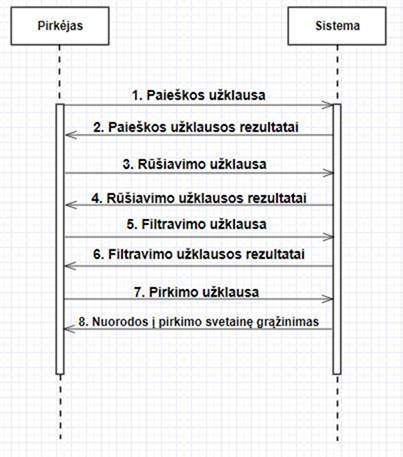
\includegraphics[scale=1]{img/paieska1}
  \caption{Paieška}
  \label{paieska}
\end{figure}

\sectionnonum{Išvados}
Vartotojo interfeiso reikalavimai leidžia suprasti, kaip turėtų atrodyti sistema – ji būtų patogi naudoti vartotojui. Funkciniai reikalavimai leidžia suprasti, kokias funkcijas ir užduotis turi atlikti programa. Nefunkciniai sistemos reikalavimai - implementacijas, aspektus. Taigi, anksčiau paminėti reikalavimai padeda suprasti, kokia sistema reikalinga vartotojui.

\sectionnonum{Terminų žodynas}
...

\printbibliography[heading=bibintoc]  % Šaltinių sąraše nurodoma panaudota
% literatūra, kitokie šaltiniai. Abėcėlės tvarka išdėstomi darbe panaudotų
% (cituotų, perfrazuotų ar bent paminėtų) mokslo leidinių, kitokių publikacijų
% bibliografiniai aprašai.  Šaltinių sąrašas spausdinamas iš naujo puslapio.
% Aprašai pateikiami netransliteruoti. Šaltinių sąraše negali būti tokių
% šaltinių, kurie nebuvo paminėti tekste.

\appendix  % Priedai
% Prieduose gali būti pateikiama pagalbinė, ypač darbo autoriaus savarankiškai
% parengta, medžiaga. Savarankiški priedai gali būti pateikiami ir
% Priedai taip pat numeruojami ir vadinami. Darbo tekstas
% su priedais susiejamas nuorodomis.

\section{Paveiksliukas}
\begin{figure}[H]
  \centering
  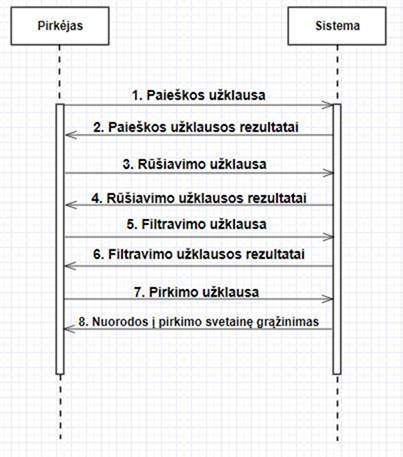
\includegraphics[scale=1]{img/paieska1}
  \caption{Paieška}
  \label{paieska}
\end{figure}

\end{document}
